\section{Technical Approach}
To infer information about Java code we use existing inference tools and
combine their output. We have additionally developed a simple framework to aid
in writing our own analyses.

To combine the results of disparate analyses we have to convert their results
into a common format at some point in our toolchain.  We will use the JAIF
(Java Annotation Index File) format for that purpose.  Some anaylses generate
results directly in JAIF format, some provide annotated bytecodes which can be
easily extracted into JAIF format, and others provide textual results for which
we will read the results into a our framework.

\begin{figure}
\centering
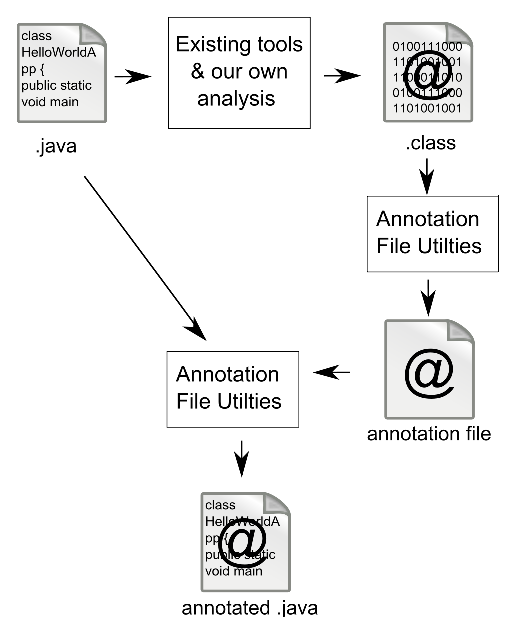
\psfig{file=figures/technicalApproach/technicalApproach.eps, width=3in}
\caption{Toolchain}
\label{fig:toolchain}
\end{figure}

In the following section we describe our analysis framework and how we
integrate all the tools into JavaGrok

Figure \ref{fig:toolchain} shows the stages in our toolchain.

\subsection{Analysis Framework}
\label{ss:analysisFramework}

To implement our own analysis tools we use the Annotation Processing Tool (APT)
API~\cite{apt} built into the Java standard compiler.  From within an APT plugin
we can access the compiler's abstract syntax tree and augment the generated
bytecode with annotations representing our analysis results. These annotations
are then extracted into external annotation files.

\subsection{From JAIF to HTML documentation}
\label{sec:jaif2html}

Once the results of the various analyses have been collected into a set of
annotation files, we use the annotation file utilities~\cite{AFU} to merge
those annotations back into the original library source. Of course this source
can now be used either directly by looking at the annotated source code. But
we also let javadoc run over the source code to generate html documentation
which now include our annotations.
